\documentclass[11pt]{article}

\usepackage[]{graphics}
\usepackage{natbib}
\usepackage{rotating}
\usepackage[margin=2cm]{geometry}
\usepackage{pgfgantt}

\usepackage{csvsimple}
\usepackage{caption}
\usepackage{subcaption}
\usepackage{url}
\usepackage{pdfpages}

%opening
\title{Developing an Intelligent Chatbot: the First Interim Report}
\author{Group UG14: Daniel Willis, Charlotte Anderson and Brandon Gous}

\begin{document}
	
	\maketitle	
	\begin{abstract}
		The report shall introduce some background to the subject as well as the groups motivations for creating the chatbot. It then discusses the group's aims, objectives and difficulties for both part 1 and 2 of the brief. In section \ref{RelatedWork}, similar systems are discusses and evaluated by their relevance to the project. In part \ref{Methods} methods, tools and frameworks used for this project are stated and explained. The design in section \ref{Design} and implementation in section \ref{Implementation} are then outlined in subsections of the different areas of work. Testing for this project is then covered briefly in section \ref{Testing}. Finally, the groups work is evaluated and concluded in section \ref{Evaluation}.
		
	\end{abstract}
	
	\section{Introduction}
	
	For this coursework \citep{AI2018CW} the group is developing an intelligent chatbot for customers to use which will find them the cheapest train ticket for a specified journey. The service shall also provide users with information on train delays, for a specified journey, to improve customer service. The chatbot will be able to recognise which service the user wishes to use, using Natural Language Processing (NLP) techniques. The chatbot will respond appropriately until it has gathered all information needed to answer the user's query.	
	
	\subsection{Background and Motivation}
		
	Increasingly chatbots are used for customer service by companies and businesses. The first wave of chatbot systems could only recognise questions posed to them if they were written exactly as it was programmed to understand \citet{Ebi}. Artificial intelligence is a hot topic at the moment, and has been used to develop seriously intelligent chatbots. Using AI, chatbots are able to understand and answer customer questions, which can be asked in a huge variation of ways. As chatbots these days are so capable, many companies favour using AI for customer service over an employee, as it can save money and time. Furthermore \citet{Sintef} found in his study than many users do understand that chatbots work best when asked direct and precise queries; therefore often the user is doing some of the work for the chatbot by using simple language.	
	
	\subsection{Aim and Objectives of this coursework} 
	The aim of the group is to develop a prototype intelligent chatbot system that can be extended to handle a large variation of queries. The chatbot will have two functions:
	\begin{enumerate}
		\item Finding a user the cheapest ticket for a specified journey.
		\item 	Reporting to a user the predicted train delay when prompted with their journey and current delay.		
	\end{enumerate}	

	Our objectives are:
	\begin{enumerate}
		\item To keep to our outlined project plan in the Gantt Chart.		
		\item Have two weekly meetings on Microsoft Team to update the group on progress made.		
		\item Have all set separate work completed for the chatbot, ready to be integrated with each other, by the 10th of January. This will give the group a week to integrate their systems together and iron out any issues, ready for the demonstration and video.
	\end{enumerate}	
	
	\subsubsection{MoSCoW Analysis}
	Must:
	\begin{itemize}	
		\item The chatbot must be able to handle single-way tickets.		
		\item The chatbot must prompt the user until enough information is obtained to complete their query.
		\item The system must be able to use the gathered information to complete the request. 
		\begin{itemize}
			\item In the case of a cheapest ticket query, it must return the cheapest ticket found and a hyperlink to a page where the customer may purchase it.
			\item In the case of prediction, it must return the predicted train delay in minutes at the users destination station.			
		\end{itemize}		
		\item Once the chatbot has received all the information it needs to search, it must check with the user it has understood the query correctly, so changes can be made if needed.
	\end{itemize}
	Should: 
	\begin{itemize}
		\item The chatbot should be able to handle return tickets.		
		\item The chatbot should be able to handle a large query with multiple pieces of information within it.
		\item The chatbot should be able to handle misspelt station names.
		\item That chatbot should return the user an answer to their question, once all the information is obtained, within 15 seconds.		
	\end{itemize}
	Could:
	\begin{itemize}
		\item The chatbot could be able to handle multiple date and time formats.		
		\item The chatbot could be able to ask the user if there is anything more they can help with.
		\item The chatbot could have an attractive user interface.
		\item The chatbot could search for multiple adults or children.				
	\end{itemize}
	Won't
	\begin{itemize}
		\item The chatbot won't be able to handle all query formats.
		\item The chatbot won't be able to recognise badly spelt station names.
		\item The chatbot won’t be able to use railcards in its search for the cheapest tickets.		
	\end{itemize}	 
	
	\subsection{Difficulties and Risks}
	
A risk with this task could be poor project management. To try and reduce this risk, in our first group meeting we decided upon a group leader, Dan. Dan ensured that we had weekly meetings in which he encouraged us to all share what we’d been working on. A large portion of this work had to be completed over the Christmas break. It was important that the team continued to work together despite not being on campus at university. Our group continued to have regular meetings on teams during this time, with the intention that this would reduce the risk of slippage in the project. 

Another risk is that deadlines will not be met. A member of the group not meeting a specific deadline could mean that the next piece of work cannot be started. To reduce this risk, the work was divided in such a way that each member could get on with a specific part of the brief. The work was delegated as follows:


Dan:
\begin{itemize}
	\item Project manager
	\item Create the database
	\item Research predictive models
	\item Programme a few of these models and report back the most successful model
	\item Work with Brandon to get this work integrated with the chatbot.
\end{itemize}
Charlotte:
\begin{itemize}
	\item Write the webscraper for the cheapest ticket
	\item Decided on the flow of conversation for the chatbot
	\item Write the NLPU component and work with Brandon to get this integrated with the chatbot.
\end{itemize}
Brandon: 
\begin{itemize}
	\item Write the Knowledge-Base
	\item Reasoning Engine and User Interface. 
	\item Worked with the other team members to get their contributions integrated with the chatbot. 
\end{itemize}

Working this way meant that each member could begin programming without having to wait for another member of the group to have already finished a task. In the weekly meetings everyone shared what they had been working on since the last. 

Once the individual work was complete the final risk was that our work would not be integrated together in time. This is a large and integral task, if all elements work separately but cannot work together the brief has not been met; for this reason one of the objectives was to begin integrating work by at least the 10th of January.
	
	\subsection{Work Plan}	
	\clearpage
	\begin{figure}{Project Gantt chart \label{pplan}}
			\begin{ganttchart}[x unit=0.35cm, y unit chart = 1.0cm, y unit title=0.5cm, title height=1.0, vgrid, title label font=\scriptsize,
				canvas/.style={draw=black, dotted},
				/pgfgantt/milestone left shift = 0,
				/pgfgantt/milestone right shift = 0
				]{6}{18}
				
				\gantttitle{Project schedule week numbers}{13} \\
				\gantttitlelist{6,...,18}{1}\\
				\gantttitlelist{6,...,12}{1}
				\gantttitle{CB}{4}
				\gantttitle{AP}{2}\\
				
				\ganttbar{Asses what needs to be done}{6}{8}\\%elem0  
				\ganttbar{Design}{8}{9}\\%elem0
				\ganttbar{Create Scraper}{10}{11}\\%elem0	
				\ganttbar{Predictive Models}{10}{13}\\%elem0
				\ganttbar{Create UI}{12}{12}\\%elem0	
				
				\ganttbar{Create Knowledge Base}{13}{14}\\%elem0	
				\ganttbar{Develop Natural Language Processing}{13}{14}\\%elem0	
							
				\ganttbar{Report Writing}{7}{8}
				\ganttbar{}{15}{17}\\%elem0		
				
						
				\ganttmilestone{Progress Check}{12}\\%elem8 
				\ganttmilestone{Due Date}{17}\\%elem8  
				
				\ganttlink{elem0}{elem1}				\ganttlink[link mid=.25]{elem1}{elem2}
				\ganttlink[link mid=.25]{elem1}{elem3}
				\ganttlink{elem2}{elem4}
			\end{ganttchart}
	\end{figure}
	\section{Related Work} \label {RelatedWork}
		
	\subsection{TFL chatbot}
	The TFL chatbot was very friendly and said “You're welcome” (or equivalent) when you thanked it \citet{TflTravelBot}. It seemed to understand what was meant most of the time very well even when the input was not very specific. It was functionally useful as it could give live information about the next few buses if it knew the stop code for the bus stop that the user was standing by. It was fully integrated with facebook messenger so it is as easy as sending a facebook message.
	
	Unfortunately it had very limited functionality especially for the tubes. Often it failed to select the correct station or it took a few attempts to get the correct station. For where there are two stations named similarly it did not offer suggestions of stations to the user to pick from. Planning was impossible as there was no way to enter a time, it only handled current time rather than a time in the future. Additionally, it couldn't understand a user if all information was entered in one message, it had to separate the too and from stations.
	
	Overall the chatbot worked well, but needed more functionality as it would only occasionally misunderstood. However, for tubes it could only tell the user what line the closures are on so, and the user has to decide if they want to see in more detail when/where they are. Additionally, a lot of the time when trying to extract information, especially when talking about cost, the chatbot would just send a link to the TFL website. 
	
	\subsection{BlenderBot}
	Blenderbot or parlai is a open source, highly customisable chatbot developed by Facebook \citet{roller2020recipes}. Its relatively easy to install and use in the terminal, and if desired it comes with integration into Facebook messenger. 
	
	One can be assigned a random persona, set one manually, or just have a general conversation. This was very interesting to play around with, giving the chatbot different characters to play with and seeing how well it handled them. 
	
	Models can be uploaded from the ``zoo", or one cane be created built off a base. The 80 million data points model is a little clunky and not as fluent. There is a definite pattern to its responses. The top level 9 billion data point weights is very impressive, and could almost pass as a human. 
	
	It's very factual too, it will attempt to slip in facts in a "normal" manner rather than just blurting them out robotically. 
	
	It comes with a lot of documentation and a paper about how to build a good model. 
	
	Overall it was entertaining and enjoyable to speak to. If there was more time for this project, this is a great feature the group would have liked to incorporate it into the project.
	
	\subsection{Google Assistant}
	Google assistant is arguably a chatbot, it commonly has a speech to text, and text to speech software alongside \citet{Google Assistant}. However there is the option on phones to just type text to it and reply, but this conversation would be the same if verbal.
	
	Google assistant is useful to perform tasks such as switching lights on and off, playing media, setting timers for cooking etc. But that is all it is, as it is designed to be a tool and to be as useful and functional as possible. It isn't designed to hold a conversation with a user. 
	
	This is where the assistant is lacking; its responses are very robotic, blunt and to the point. No human speaks like that. Any questions asked will have an answer from crawling the web or doing the maths. Users can ask it to tell them a joke, ask about the weather, or how the traffic looks on your morning commute, but it cannot hold a conversation; it is being used as a tool to solve a users problem.
	
	Its natural language processing is near perfect and in real time from audio which is incredible. It really understands what you are saying so long as it is a command. Overall, a very useful product to have around, but not the best chatbot.	
	
	\section{Methods, Tools and Frameworks} \label{Methods}
	     
	\subsection{Methods}
	
A primarily text based user interface was selected, along with an aim to wrap the text-based system in a graphical user interface. The user’s responses would be processed using a natural language processing library called Spacy. From the responses provided by the user, the knowledge engine would determine what steps are next based on rules built into the system and which of those match the user’s responses.


For the delay prediction we used a K-Nearest-Neighbour (KNN) method and a neural network. 
	
	\subsection{Languages, Packages, Tools}
	
	The two main languages that were selected were Python and C\# for the main chat-bot and then some of the database interaction respectively.
	Within the chatbot the following packages were used:
	\begin{itemize}
		\item Experta - Used for the knowledge engine, it handled all of the questions relating to the state of the booking/delay prediction query.
	\item Fuzzywuzzy - Used to process station names that may have been entered incorrectly. Such as in the case of typos.
	\item Datetime - Was used for reading and formatting dates.
	\item Spacy - Spacy was used for all of the natural language processing.
	\item Json - JSON was the format that the text stemming was stored in, so the library was used to read and understand that.
    \item Pandas - Pandas is a data analysis library that we used to help round some timing to better work with the train data.
	\item Selenium - Was a web-scraping library that we used to extract data from websites to feed back to the user 
	\item Numpy - Was used for most of the arrays in the delay prediction, and the matrix transformations required.
	\item Matplot - Was used for the graph plotting so that we could visualise how the two delay prediction methods were working and compare them.
\end{itemize}
	For the database, we selected SQL Express. Because a member of our group had used this a lot on their placement year so was familiar with MYSQL.	   
	
	%\subsection{Development Framework}	
	
	\section{Design of the Chatbot}	 \label {Design}
	
	\subsection{The Architecture of the chatbot}
	
	In an early group meeting we decided to conduct the work for this project modularly. This meant creating contracts with one another on what work would be completed by each member, by when and detailing exactly what we expected from each piece of work. This meant we could work separately, which was necessary as much of this work was completed away from university. It was decided that Dan would create a database, as well as writing predictive models, Brandon would write the knowledge-base and inferring engine, and Charlotte would write the scraper and Natural Language Processing Unit (NLPU). Once all this work was completed, the group could come together and integrate the various pieces of work. 
	
	
	The chatot is responsible for handling questions from a user and responding to these. It uses the NLPU to understand what a user has inputted, as well as to see if all fields have been filled for a search. If all fields have not been inputted, the chatbot will reply to the user asking for the information it is missing. Once the NPLU has all the information it needs to make a search, it delivers this to the scraper, or the prediction model depending on the task. If the task is for find the cheapest ticket, once this has been found the chatbot will relay this information to the user with a price and a link to buy the ticket. Similarly, for predicting train delays, once the predicted delay has been predicted, it is relayed through the chatbot to the user.
	
	\subsection{User Interface} 
	For the user interface, we decided to emulate a chat window similar to your typical messaging app, consisting of a chat log, chat line and send button. The chat log would display a history of all the messages sent between the user and the chatbot, whilst displaying who sent each message and the time sent. The chat line and send button would be the way the user interacts with the system. Responses to messages sent by the chatbot would be written in the chat line and then “sent” for processing when the return key, or the send button are pressed.	
	
	
	\subsection{Scraper}
	The scraper will input all necessary fields in Trainline’s website. Trainline’s ticket search will fail if the train station is spelt wrong so the scraper needs to work with the NLPU to ensure stations are correctly spelt. Additionally, the website only handles specific date formats so the NLPU will need to format differing date formats into the accepted version.
	
	\subsection{NLP}
	The NLPU shall be able to handle large queries. This means a user can input into the chatbot a sentence with lots of information in, and the NLPU shall be able to understand what the user is asking for. This may not be achievable for all structures of sentences as that would be very complicated, but annexs \ref{appendix:ChatFlow} shows the structure of a sentence the NLP will be designed to work for. The NLPU shall also accept multiple date formats, time formats and understand words like ‘tomorrow’ and ‘today’.
	
	
	\subsection{Knowledgebase and Inferring Engine}
	The knowledge base will handle getting all of the information it requires from the user through the use of the inferring engine. The knowledge base will get information from the user in the form of questions, and the inferring engine will use a set of conditions to determine which question needs to be asked and when. The set of conditions will evaluate which information has been obtained from the user, the validity of the information, and what information is missing.
	
	\subsection{Delay Prediction Models}
	
	Three prediction models are planned to be tested. A Bayesian model that calculates the probability of the train being late to the second station, given that the train is delayed to the first station. A neural network that uses the delay and the normal time a train takes between the stations to predict how late the train will be. And KNN which predicts how late the train will be to the second station using similar data.
	
	\subsubsection{Bayesian}
	
	Bayesian Theorem is that the probability of event A happened given that B happened can be calculated by the probability of event B happening given that event A happened multiplied by the probability of event A happening all divided by the probability of event B happening.	
	\[P(A|B) = \frac{P(B|A) * P(A)}{P(B)}\]
	
	Additionally this can be expanded so that the probability of event B happening doesn't need to be known. 
	The probability of event B happening is equal to the probability of event B happening, given event A happened multiplied by the probability of event A occurring, plus the probability of event B happening given that event A does not, multiplied by the probability that event A does not happen.
	
	\[P(B) = P(B|A) * P(A) + P(B|'A) * P('A)\]
	
	This means that the probability of event A happening, given that B happened, can be calculated from the probability of event A happening, the probability of event B happening given event A happened, and the probability of event B happening given that event A didn't happen.
	\[P(A|B) = \frac{P(B|A) * P(A)}{P(B|A) * P(A) + P(B|'A) * (1 - P(A))} \]	
	
	This is applied to the prediction of trains being late by letting event A be the train being late to the second station, and the event B being the the train being delayed at the first station.
	
	\subsubsection{Neural Network}
	
	A neural network is a collection of layers of neurons, each neuron holds a value known as activation of that neuron. There can be an unlimited number of layers and neurons and they can be used to solve very complex problems such as object recognition.
	
	Each neuron is connected to all the neurons of the previous layer through numbers called weights (W) and a bias (b). The weights are organized in the form of a matrix of the shape number of units in current layer by number of units in previous layer. This means that to calculate a neuron on the next layer, all the previous values are needed.
	
	If this is applied to the project there would be, two input nodes; one for the delay at the first station, and one for the normal time taken between the stations. And there is one output node for the prediction time that the train is late. These two layers cannot be changed change, but any of the hidden layers can be altered to still produce a neural network to accomplish the same goal. This is shown in figure \ref{Img:NNDiagram} it shows all the neurons in the simple neural network that has been designed to solve the problem with two hidden layers of three neurons each.
	
	\begin{figure}[!htb]
		\begin{center}
			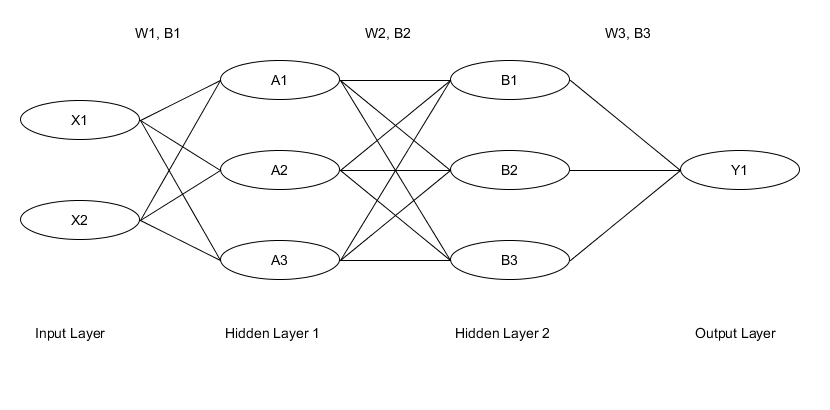
\includegraphics[width=1\textwidth]{Resources/PartTwo/NNDiagram.png}
			\caption{Diagram showing the neural network}
			\label{Img:NNDiagram}
		\end{center}
	\end{figure}
	
	For the maths behind the forward and backward propagation, Wk\textsubscript{ij} refers to the weight of the connection from i’th neuron in k'th layer to j’th neuron in k-1 layer. The biases are organized in the shape of (no. of units in current layer, 1) so Bk\textsubscript{i} corresponds to the bias of the i’th neuron in k'th layer. 
	
	Each neurons value can be calculated by:
	\[A1 = g(f(X1,X2)) = g(W1_{11}*X1 + W1_{12}*X2 + b1_{1})\]
	\[A2 = g(f(X1,X2)) = g(W1_{21}*X1 + W1_{22}*X2 + b1_{2})\]
	\[A3 = g(f(X1,X2)) = g(W1_{31}*X1 + W1_{32}*X2 + b1_{3})\]
	
	\[B1 = g(f(A1,A2,A3)) = g(W2_{11}*A1 + W2_{12}*A2 + W2_{13}*A3 + b2_{1})\]
	\[B2 = g(f(A1,A2,A3)) = g(W2_{21}*A1 + W2_{22}*A2 + W2_{23}*A3 + b2_{2})\]
	\[B3 = g(f(A1,A2,A3)) = g(W2_{31}*A1 + W2_{32}*A2 + W2_{33}*A3 + b2_{3})\]
	
	\[Y = f(B1,B2,B3) = W3_{11}*B1 + W3_{12}*B2 + W3_{13}*B3 + b3_{1}\]
	
	Where $g(x)$ is the activation function. Being as this is a regression problem and not classification $g(x) = max(0,x)$ is used, and is more commonly called the ReLU. This returns 0 when $x$ is negative and $x$ when positive. Due to it’s low saturation region, it is highly trainable. 
	
	The equations above can be vectorised using the dot product of the matrices:
	
	\[A = g(W1.X + b1)\]
	\[B = g(W2.A + b2)\]
	\[Y = W3.B + b3\]
	
	However for the neural network to become more accurate it has to learn by adjusting the weights an bias to bring the output closer to the target. This is done using a back propagation algorithm to calculate the gradients. These are the vectorized equations:
	
	\[dY = \frac{1}{m} * (Y-T) \]
	
	\[dW3 = \frac{1}{m} * (dY.W3^T) \]
	\[db3 = \frac{1}{m} * \sum dY \]
	\[dB = W3^T.dY\]
	
	\[dW2 = \frac{1}{m} * (dB.W2^T) \]
	\[db2 = \frac{1}{m} * \sum dB \]
	\[dA = W2^T.dB * g'(W2.A+b2)\]
	
	\[dW1 = \frac{1}{m} * (dA.W1^T) \]
	\[db1 = \frac{1}{m} * \sum dA \]
	
	Where T is the true value, $m$ is the number of datapoints, $*$ is multiplication, $x.y$ is dot product of the matrices $x$ and $y$ and $x^T$ is the transpose of matrix $x$. We do not need gradients with respect to the input layer neurons because they are not going to be changed.

	Now using these gradients calculated, weights can be modified, as well as bias, which gets a result closer to what the true result would be.
	
	\[W1 = W1 - lr * dW1\]
	\[b1 = b1 - lr * db1\]
	\[W2 = W2 - lr * dW2\]
	\[b2 = b2 - lr * db2\]
	\[W3 = W3 - lr * dW3\]
	\[b3 = b3 - lr * db3\]
	
	Where $lr$ is the learning rate which is a configurable hyperparameter that is in the range between 0.0 and 1.0. The learning rate controls how quickly the model adapts to the problem.
	
	\subsubsection{K Nearest Neighbors}		
	
	For the K nearest neighbour model lots of data has been extracted from the database for each query. A stored procedure has been used for this.
	
	The amount the train was late to the first station in the historical data, is then compared to the amount of delay that the user had at the first station using a distance function; in this case euclidean distance is used.
	
	These distances are then sorted and you get the mean of the delay at the second station for the closest K nodes in the dataset. This is simple algorithm, but heavily dependant on finding the correct K value. Too small, and the correct number will not be found  it will be skewed as there isn't enough data, or it is too large and the result will be skewed by nodes that are not close enough.
	
	%\subsection{Conversation Control}
	
	%\begin{table}
		%\centering
		%\caption{This table lists ......}
		%
		%\begin{tabular}{|c|c|c|c|c|c|}
			%\hline Methods &  &  &  &  &  \\ 
			%\hline  &  &  &  &  &  \\ 
			%\hline  &  &  &  &  &  \\ 
			%\hline 
			%\end{tabular} 
		%\label{TableCC}
		%\end{table}
	
	\section{Implementation} \label{Implementation}
	
	\subsection{Scraper}
	The implementation of the scraper has been designed to complete the task of finding a cheapest ticket for a train booking. Trainline’s website \citet{trainline} was chosen to be scraped, this was because when inspecting the page when a search was completed there was a clear tag which indicated the cheapest ticket which could then be used to return to the user. The package `selenium’ \citet{selenium} was used to webscrape as it was found to be the most useful for what was trying to be achieved. The TrainLine class has many functions which find different elements within TrainLine’s page, which are then filled once the chatbot has retrieved information from the user. 
	
	The scraper clears all field boxes before entering data. This is because if a field was pre-filled by the website, i.e. defaulting to today's date, when the scraper tried to enter the date which has been specified by the user, it cannot do so as it is already full and throws an error. The scraper uses selenium to find specific elements within the page that will be filled with the users query. For example if a user wants a single ticket, it is capable of choosing between the radio buttons for a `single’ or `return’ journey. This is done by using TrainLine’s element ID’s, for example the radio button for a single tickets element ID is `single’, and therefore can be found and clicked. 
	
	Once a full search has been made, the scraper waits for an element with an `aria-label’ that has the value `the cheapest fare’. The price which belongs to this value is the cheapest ticket for the specified journey, and this price and the link to the page is given as a reply to the user through the chatbot.	
	
	\subsection{NLP}
	The NLPU is essential to the scraper. TraineLine’s website only works for certain date formats, 24 hour times, full and correctly spelt train stations, and will only complete a search successfully if it has all of the information. The NLPU works with the chatbot to ensure all fields are full before passing this information to the scraper so it doesn’t fail. Not only this, but the chatbot has to be able to understand what a user is asking it to do. The NLPU can identify, using SpaCy’s \citet{Spacydoc} parts of speech, when a user is inputting a cheapest ticket query or prediction query. It does this by looking for specific words in the sentence. To identify whether it is a cheapest ticket query it looks for words in the stems.json file, which matches similar words. If a query contains the a words, once stemmed,  `book’, `ticket’, `cheap’ or `buy’, it infers that the user is wanting to find the cheapest ticket, rather than asking about a delay prediction. The same goes for the prediction query.

	One of the most important parts of the NLPU for this project was the chatbot recognising train station names that were spelt incorrectly, or missing parts of the station name, as when these stations are inputted into the scraper they must be exact or the search will not run. To do this a package called ‘fuzzywuzzy’ was used, which does a ‘fuzzy match’ on station names and finds percentage matches to the station names inputted. If a station is not a 100\% `fuzzy match’, the chatbot suggests any station that has an 85\% match or higher. The unit also handles multiple different date formats, times and understands words like ‘today’ and ‘tomorrow’.

	\begin{figure}[!htb]
		\begin{center}
			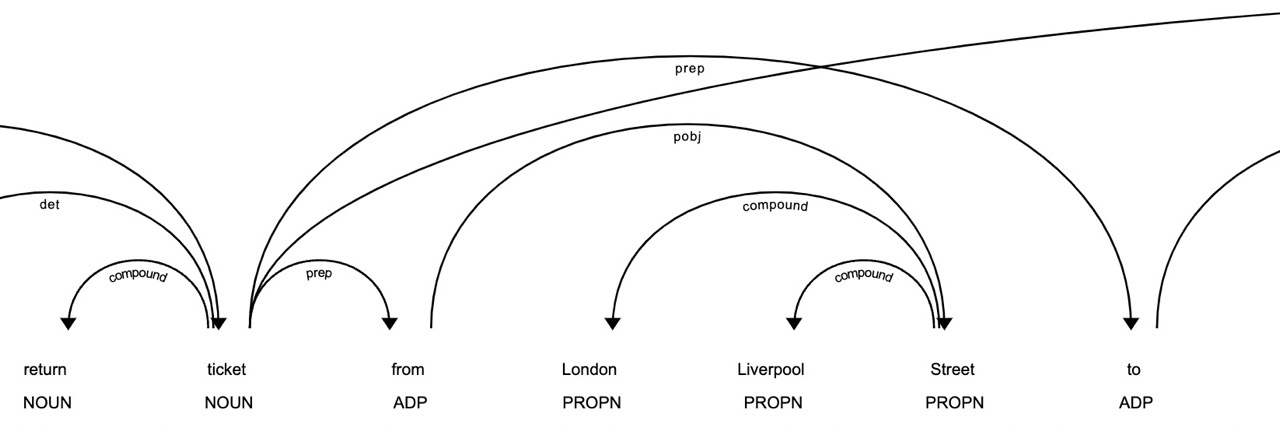
\includegraphics[width=1\textwidth]{Resources/partsOfSpeechLarge.jpeg}
			\caption{Example of SpaCy's parts of speech tagging on a cheapest ticket query}
			\label{Img:Spacy}
		\end{center}
	\end{figure}

	For sentence queries, like the one in figure \ref{Img:Spacy}, the NLPU works by using SpaCy, looking at parts of speech tags like `NOUN' or `VERB' or for words within the stems.json file. For example, if the parts of speech tag is `ADP' and one of the relating `from\_station' words in the stems.json file, the program extracts the following station name and sets it to the origin station.

	\subsection{KnowledgeBase and Inferring engine}
	The knowledge base and inferring engine were implemented with a library called Experta. Experta will store declared facts, such as where the user wants to go, or where they are coming from.

	From the declared facts, the engine will infer which function should next be run based on rules associated with each. The rules will be evaluated, and if true the function runs. In the case of multiple rules being evaluated to be true, the engine will pick a random one.

	After each function is run, all of the rules are re-evaluated so an updated set of available functions is available for selection. Once there are no remaining functions, the application will terminate.

	\subsection{Predictive Models}

	\subsubsection{Bayes}
	To get the probabilities we can use stored procedures to extract the frequencies from the database.

	Firstly the probability of A (the train being late to the second station)  was easy enough to calculate as I simply extracted the frequency count of all the times the train arrived at the second station late and divided by the total pieces of data I had.

	Secondly I calculated the probability of B given A (the probability the train was late to the first station by delay given it was late to the second station). To do this I extracted the frequencies of delays at the first station if the train arrived late to the second station. From here I summed all the frequencies that the train was late to the first station by at least the delay.

	Next I calculated the probability of B given not A (the probability the train was late to the first station by delay given it was on time to the second station). To do this I extracted the frequencies of delays at the first station if the train arrived on-time or early to the second station. From here I summed all the frequencies that the train was late to the first station by at least the delay, then it was just a case of doing the calculation and returning the result as a probability.

	\subsubsection{Neural Network}

	 We thought that the best way to implement all the weights and values being stored was through dictionaries with string keys eg: "W1" with multidimensional arrays as the value.

	 This meant that I could implement a solution which has the capacity to expand the number of layers and neurons per layer easily with simple for loops, making the solution highly customizable.

	 To keep track of how well the network was learning we would test every single data point through it every 1000 iterations and get the root mean squared error (RMSE) for them all. This was then plotted on a graph seen in figure \ref{Img:NNTrainA}. This shows how quickly it could correct itself at the start and then converge to 0 with a shape similar to $y=x^{-1}$ graph. This was the shape that we expected to see.

	 \begin{figure}[!htb]
	 	\centering
	 		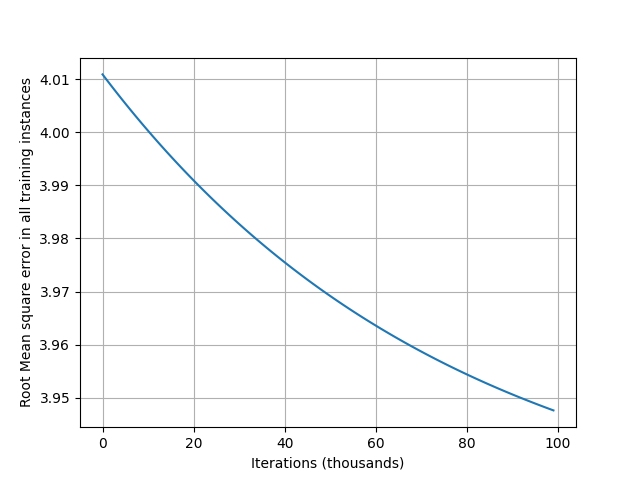
\includegraphics{Resources/PartTwo/LearningGraphs/20220111_184633_1000_1.png}
	 		\caption{Comparison of neural network and K nearest neighbour}
	 		\label{Img:NNTrainB}
	 \end{figure}

 	We would also graph every hundred thousand iterations  as seen in figure \ref{Img:NNTrainB} to be able to see more clearly that is learning still. However this quickly has a very small range on the Y axis showing it is learning slower.

	\subsubsection{K Nearest Neighbour}
	Once you have the data for the KNN it is a very simple algorithm but still heavily depends on the correct K value. So to find the best K value we set up a test to run one thousand iterations of selecting random data points from the data. Then for each piece of data I would create a KNN object with a different value of K ranging 1 to 100 (inclusive). Get a prediction from each object and compare it to the target outcome. From this I calculated the root mean square error for each value of K over the iterations.

	The results plotted on a graph is in figure \ref{Img:KSearch} and the top ranking results are included in the table in figure \ref{Img:KSearchRaw}.
	The shape of the graph is exactly what I expected to see with very few neighbours having a very high RMSE and then having a dip where the ideal K value is with the RMSE gradually increasing again as the more neighbours are used.

	\begin{figure}[!htb]
		\centering
		\begin{minipage}{.8\textwidth}
			\centering
			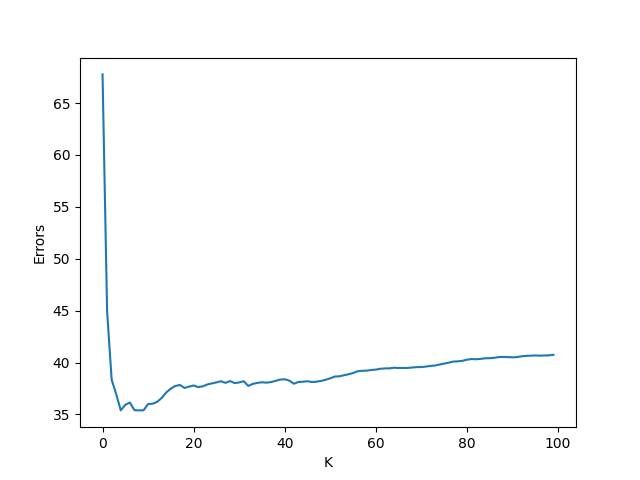
\includegraphics[width=.8\linewidth]{Resources/PartTwo/searchingForK_20220110_065714.png}
			\captionof{figure}{Searching for the correct K value}
			\label{Img:KSearch}
		\end{minipage}%
		\begin{minipage}{.2\textwidth}
			\centering
			\csvautotabular{Resources/PartTwo/KResults_Sorted.csv}
			\captionof{figure}{Sorted RMSE of K values}
			\label{Img:KSearchRaw}
		\end{minipage}
	\end{figure}

	From these results I concluded that 9 was the best value for K not only because it ranks at the top but because 10 and 8 rank 3rd and 4th in the list. However any value from 5 - 15 would still be accurate.
	\subsubsection{Comparison}
	We didn't think that the Bayesian model was very good as it is a classification model not a regression model, therefore not particularly useful to the user as they would want to know their expected time of arrival.
	
	%\begin{figure}[!htb]
	%	\begin{center}
	%		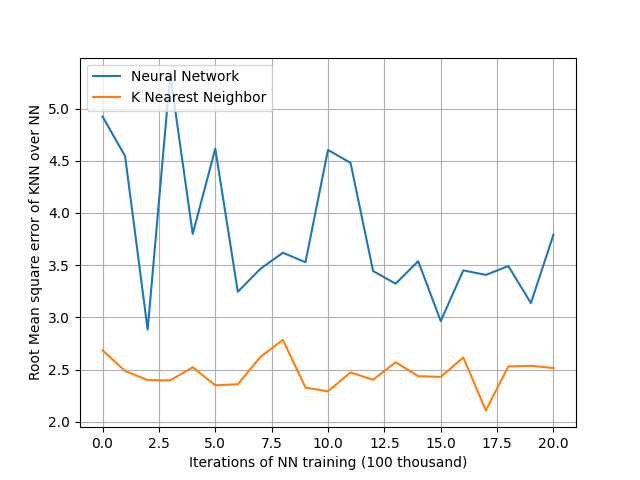
\includegraphics{Resources/PartTwo/Comparison_20220112_152958.png}
	%		\caption{Comparison of neural network and K nearest neighbour}
	%		\label{Img:NNKNNComp}
	%	\end{center}
	%\end{figure}
	
	In figure \ref{Img:NNKNNComp} we compare the neural network and k nearest neighbours over two million iterations of training the neural network.
	
	This was accomplished by randomly selecting a thousand data sets, running these datasets through both the models and comparing the predictions to the targets. Then train the neural network on the same dataset for a hundred thousand iterations and repeat.
	
	As you can see the K nearest neighbour algorithm is consistently better than the neural network despite the improvements made so we decided to use that as our final predictive model.
	
	\section{Testing} \label{Testing}
	
	\subsection{Unit Testing}
	For the predictive models and NLP, unit tests were used to check that each function achieved its intended purpose; this approach is known as test driven development. Unit tests were written first, then code was developed to pass these tests. This meant the group was able to monitor which parts of development needed more work, and which were complete. Before each merge on GitHub, these tests were run to check that the code being pushed hadn’t broken the previous commit. For the NLP, as the scope of what the chatbot could understand is massive, specific tests were written for what the group had outlined as chatflows it should accept. 
	
	
	\subsection{Integration Testing}
	
	For our chatbot all the sections are very well encapsulated through design. This also means that they only interact in the knowledge base which is where all the crossover is. 
	
	To integrate the prediction models we mapped the station names to the TIPLOC in the database that was used throughout the prediction models. This also enabled us to validate that the stations were in the correct order and actually on the line being used. Because of the way the prediction models can be encapsulated this enabled us to simply add a handful of lines of code.
	
	To integrate the NLP, all that was required was calling the correct functions when appropriate in order to process and validate the inputs provided by the user, along with appropriate messages detailing the progress towards extracting all of the information needed.
	
	Integrating the web scraper was very similar to how the prediction models and NLP were integrated. As mentioned, and as a result of the encapsulation used, the extent of it was simply calling a function and using the values returned in a message to the user.
	
	\subsection{System Testing}
	
	System testing was completed through giving the fully integrated system a variety of initial queries, along with any subsequently required inputs to see if the output is as expected and to ensure that no other information is required from the user beyond what was initially supplied.
	
	\subsection{Usability Testing}
	
	To make the chatbot more user friendly we began by anticipating the formats what we expected a user to reasonably respond to each question. If the user responded in an unsupported format we would say the format that is required. This will make it easier for the user to enter the correct data.
	
	The chatbot will also hold a conversation until the required information is collected. 
	
	The chatbot will ask very specific questions especially if the user states that the data was incorrect. This enables the user to respond correctly as they are unambiguous.
	
	In order to make itself as clear as possible the chatbot will use previous collected information in order to tailor the question making it as clear as possible in what it is asking for. 
	
	\section{Evaluation and Conclusion}\label {Evaluation}
	The scope of this project is huge and open ended, and therefore an endless amount of additions could be made to the project to make it faster and smarter. However, for the time that the group had to work on it, we are extremely happy. The chabot can handle full sentences, as well as prompting the user for any missing information. The information given to the chatbot is validated, and when appropriate the chatbot will make an attempt at what it thinks the user meant, or provide options the user can select from. The scraper is successful in finding a user the cheapest ticket for the parameters it has been given, however there is a significant delay when loading Trainline’s website, which could be mitigated if we had been granted access to National Rails API. Additionally, delays are predicted with reasonable accuracy, but with more time could be improved further. 
	
	
	In conclusion, work was completed to a high standard and as a group we are pleased with what we have produced. The individual parts of this project were challenging, as was working as a group remotely. There were a few setbacks during the course of the project due to illness and extenuating circumstances. Despite this we have created a piece of work we are all proud of, and that we believe meets the required specification. 
	
	
	\bibliographystyle{agsm}
	%\bibliographystyle{apalike}
	% you should use your own bibtex file to replace the following example_ref bib file.
	\bibliography{Referances} 
	\clearpage
	\appendix
	
	\section{Chat Flow} \label{appendix:ChatFlow}	
		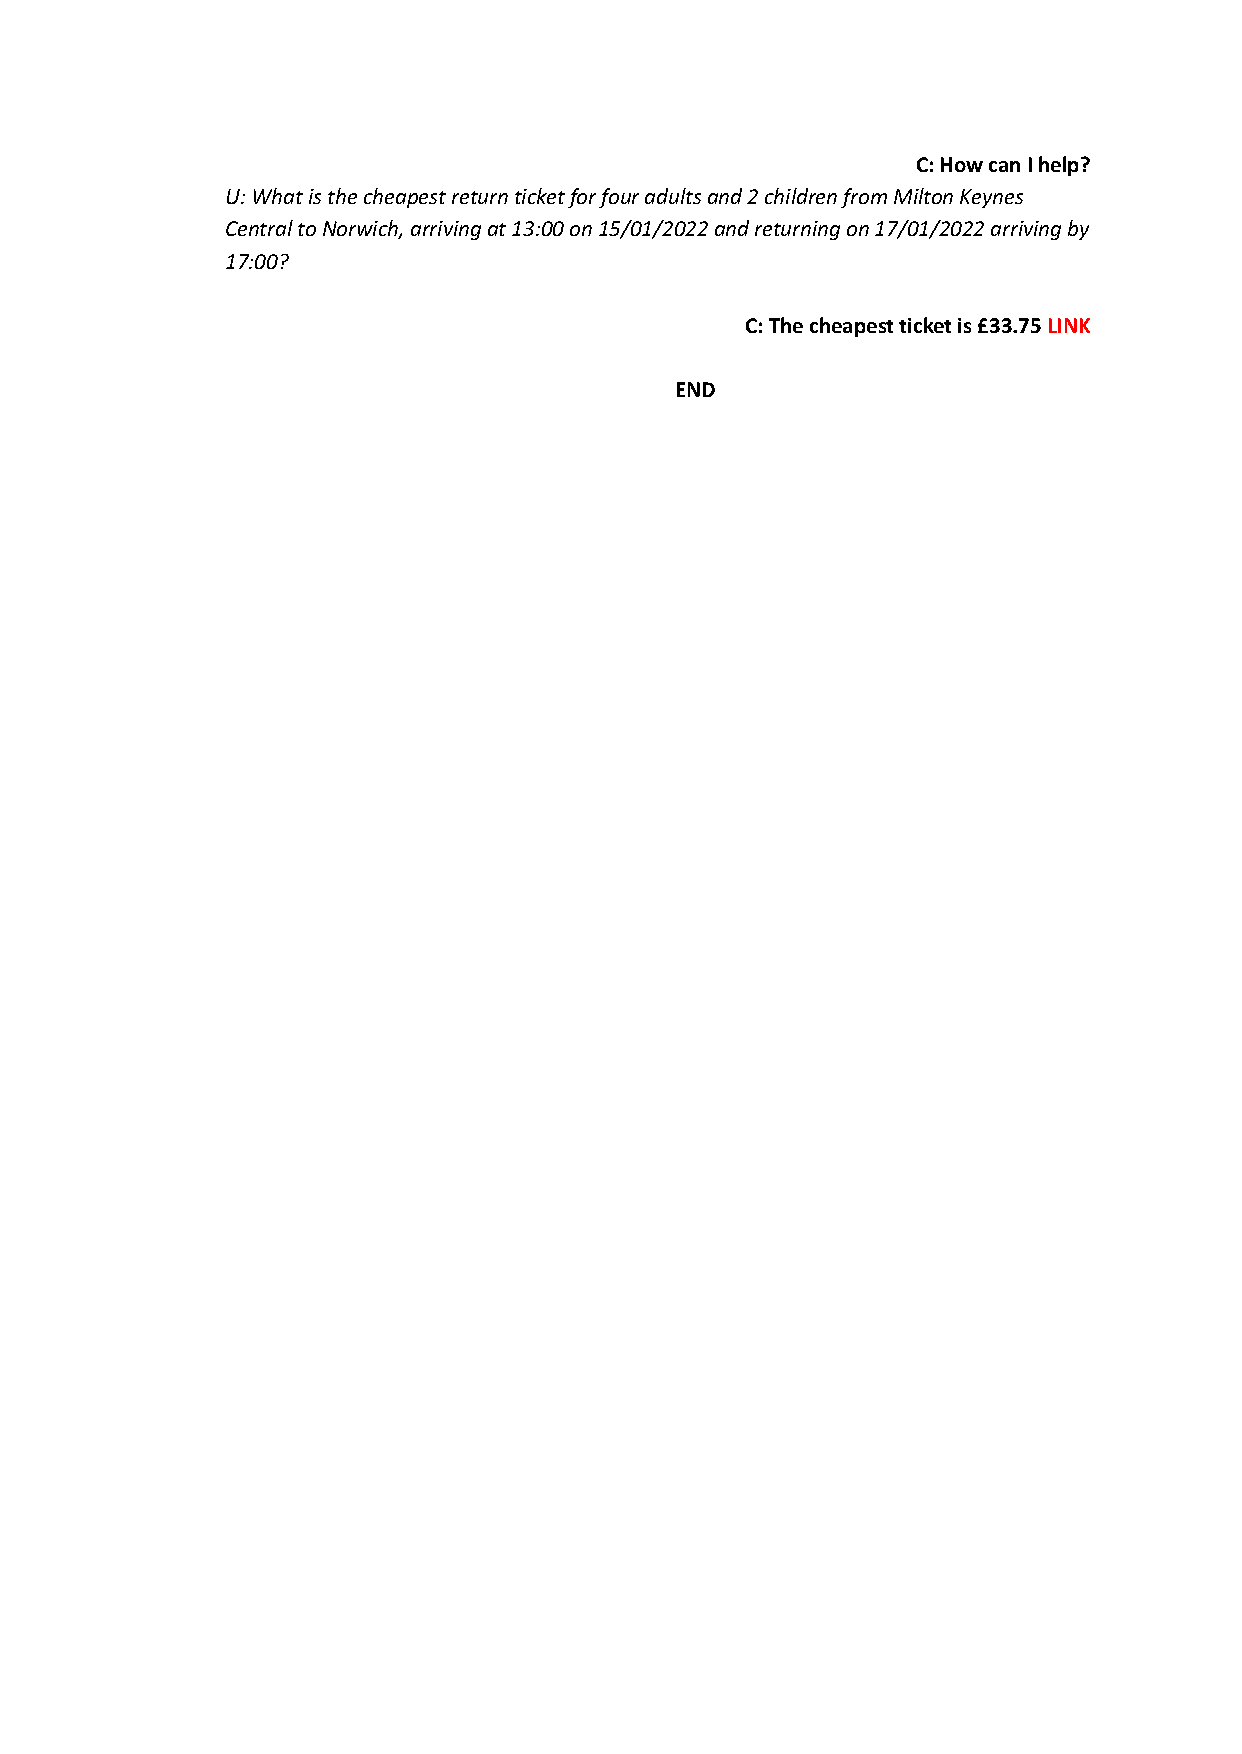
\includepdf[pages={1-4},pagecommand={\pagestyle{plain}},linktodoc=true,width=1\textwidth]{Resources/Annex/chatbotDialog.pdf}
	
\end{document}
